% Options for packages loaded elsewhere
\PassOptionsToPackage{unicode}{hyperref}
\PassOptionsToPackage{hyphens}{url}
%
\documentclass[
]{article}
\usepackage{amsmath,amssymb}
\usepackage{lmodern}
\usepackage{iftex}
\ifPDFTeX
  \usepackage[T1]{fontenc}
  \usepackage[utf8]{inputenc}
  \usepackage{textcomp} % provide euro and other symbols
\else % if luatex or xetex
  \usepackage{unicode-math}
  \defaultfontfeatures{Scale=MatchLowercase}
  \defaultfontfeatures[\rmfamily]{Ligatures=TeX,Scale=1}
\fi
% Use upquote if available, for straight quotes in verbatim environments
\IfFileExists{upquote.sty}{\usepackage{upquote}}{}
\IfFileExists{microtype.sty}{% use microtype if available
  \usepackage[]{microtype}
  \UseMicrotypeSet[protrusion]{basicmath} % disable protrusion for tt fonts
}{}
\makeatletter
\@ifundefined{KOMAClassName}{% if non-KOMA class
  \IfFileExists{parskip.sty}{%
    \usepackage{parskip}
  }{% else
    \setlength{\parindent}{0pt}
    \setlength{\parskip}{6pt plus 2pt minus 1pt}}
}{% if KOMA class
  \KOMAoptions{parskip=half}}
\makeatother
\usepackage{xcolor}
\IfFileExists{xurl.sty}{\usepackage{xurl}}{} % add URL line breaks if available
\IfFileExists{bookmark.sty}{\usepackage{bookmark}}{\usepackage{hyperref}}
\hypersetup{
  pdftitle={Instructions for Workshop Pilot},
  pdfauthor={Andrés Aguilera Castillo; Luis Carlos Castillo},
  hidelinks,
  pdfcreator={LaTeX via pandoc}}
\urlstyle{same} % disable monospaced font for URLs
\usepackage[margin=1in]{geometry}
\usepackage{graphicx}
\makeatletter
\def\maxwidth{\ifdim\Gin@nat@width>\linewidth\linewidth\else\Gin@nat@width\fi}
\def\maxheight{\ifdim\Gin@nat@height>\textheight\textheight\else\Gin@nat@height\fi}
\makeatother
% Scale images if necessary, so that they will not overflow the page
% margins by default, and it is still possible to overwrite the defaults
% using explicit options in \includegraphics[width, height, ...]{}
\setkeys{Gin}{width=\maxwidth,height=\maxheight,keepaspectratio}
% Set default figure placement to htbp
\makeatletter
\def\fps@figure{htbp}
\makeatother
\usepackage[normalem]{ulem}
% Avoid problems with \sout in headers with hyperref
\pdfstringdefDisableCommands{\renewcommand{\sout}{}}
\setlength{\emergencystretch}{3em} % prevent overfull lines
\providecommand{\tightlist}{%
  \setlength{\itemsep}{0pt}\setlength{\parskip}{0pt}}
\setcounter{secnumdepth}{-\maxdimen} % remove section numbering
\ifLuaTeX
  \usepackage{selnolig}  % disable illegal ligatures
\fi

\title{Instructions for Workshop Pilot}
\usepackage{etoolbox}
\makeatletter
\providecommand{\subtitle}[1]{% add subtitle to \maketitle
  \apptocmd{\@title}{\par {\large #1 \par}}{}{}
}
\makeatother
\subtitle{Computational Tools for Research -- Intro\\
University of Urbino\\
PhD Program in Global Studies}
\author{Andrés Aguilera Castillo \and Luis Carlos Castillo}
\date{05 April 2022}

\begin{document}
\maketitle

\hypertarget{download-and-install-reference-management-software-of-your-preference}{%
\section{1. Download and Install Reference Management Software of your
preference}\label{download-and-install-reference-management-software-of-your-preference}}

\begin{itemize}
\item
  Zotero:
  \href{https://www.zotero.org/download/}{\uline{https://www.zotero.org/download/}}
\item
  Mendeley:
  \href{https://www.mendeley.com/download-reference-manager/windows}{\uline{https://www.mendeley.com/download-reference-manager/windows}}
\item
  EndNote:
  \href{https://endnote.com/downloads}{\uline{https://endnote.com/downloads}}
\end{itemize}

\hypertarget{create-an-account-with-reference-manager-of-your-preference}{%
\section{2. Create an account with Reference Manager of your
preference}\label{create-an-account-with-reference-manager-of-your-preference}}

Register with your university email

\begin{itemize}
\item
  Zotero:
  \href{https://www.zotero.org/user/register}{\uline{https://www.zotero.org/user/register}}
\item
  Mendeley:
  \href{https://id.elsevier.com}{\uline{https://id.elsevier.com}} Enter
  email -\textgreater{} Continue
\item
  EndNote:
  \href{https://access.clarivate.com/register?app=endnote}{\uline{https://access.clarivate.com/register?app=endnote}}
\end{itemize}

\hypertarget{install-the-web-browser-plugins-for-your-preferred-reference-manager}{%
\section{3. Install the web browser plugins for your preferred Reference
Manager}\label{install-the-web-browser-plugins-for-your-preferred-reference-manager}}

\begin{center}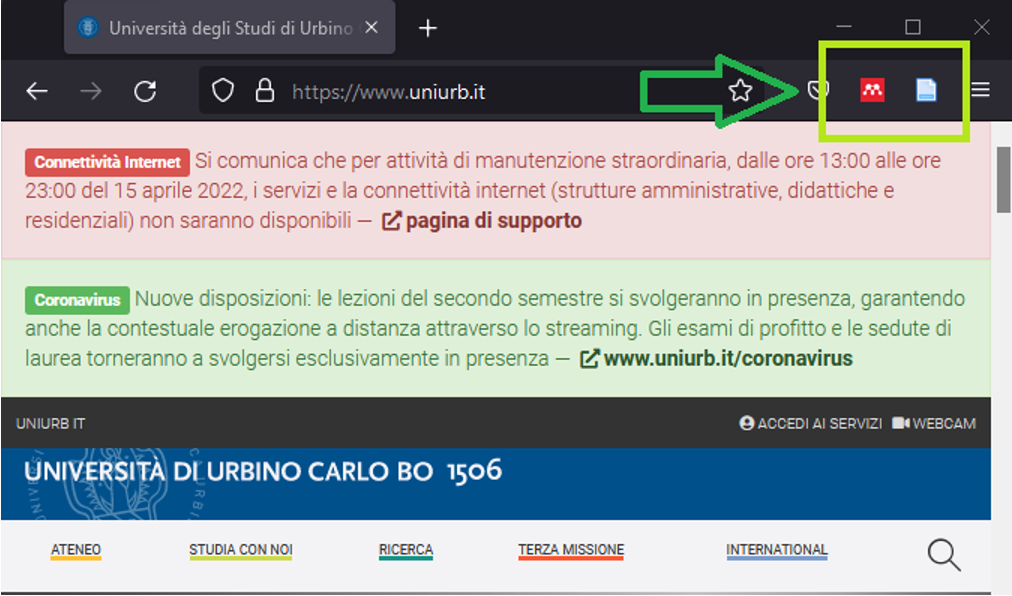
\includegraphics[width=1\linewidth]{C:/Users/eagle/Documents/GitHub/workshop_uniurb/Images/uniurb} \end{center}

Image: Example of plugin for Mendeley and Zotero in Firefox, it is also
compatible with chrome and edge.

\hypertarget{install-the-browser-plugin}{%
\section{4. Install the browser
plugin}\label{install-the-browser-plugin}}

Open your browser and go to setting -\textgreater{} extensions

\begin{itemize}
\item
  Zotero Connectors:
  \href{https://www.zotero.org/download/connectors}{\uline{https://www.zotero.org/download/connectors}}
\item
  Mendeley Web Importer:
  \href{https://www.mendeley.com/reference-management/web-importer}{\uline{https://www.mendeley.com/reference-management/web-importer}}
\item
  EndNote Capture Reference Tool:
  \href{https://support.clarivate.com/Endnote/s/article/EndNote-Capture-Reference-Tool?language=en_US}{\uline{https://support.clarivate.com/Endnote/s/article/EndNote-Capture-Reference-Tool?language=en\_US}}
\end{itemize}

\hypertarget{create-a-web-of-science-account-uniurb.it---iris-ricerca---web-of-science}{%
\section{5. Create a Web Of Science accountUniurb.it -\textgreater{}
IRIS RICERCA -\textgreater{} Web of
Science}\label{create-a-web-of-science-account-uniurb.it---iris-ricerca---web-of-science}}

\begin{center}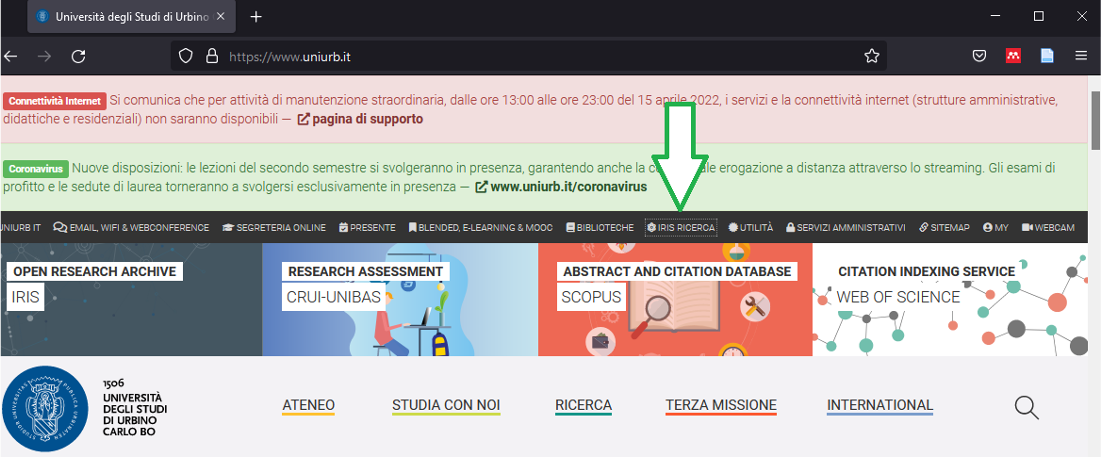
\includegraphics[width=1\linewidth]{C:/Users/eagle/Documents/GitHub/workshop_uniurb/Images/wosuniurb} \end{center}

\hypertarget{web-of-science}{%
\section{Web of Science}\label{web-of-science}}

If it is your first time in Web of Science -\textgreater{} register with
email

\begin{center}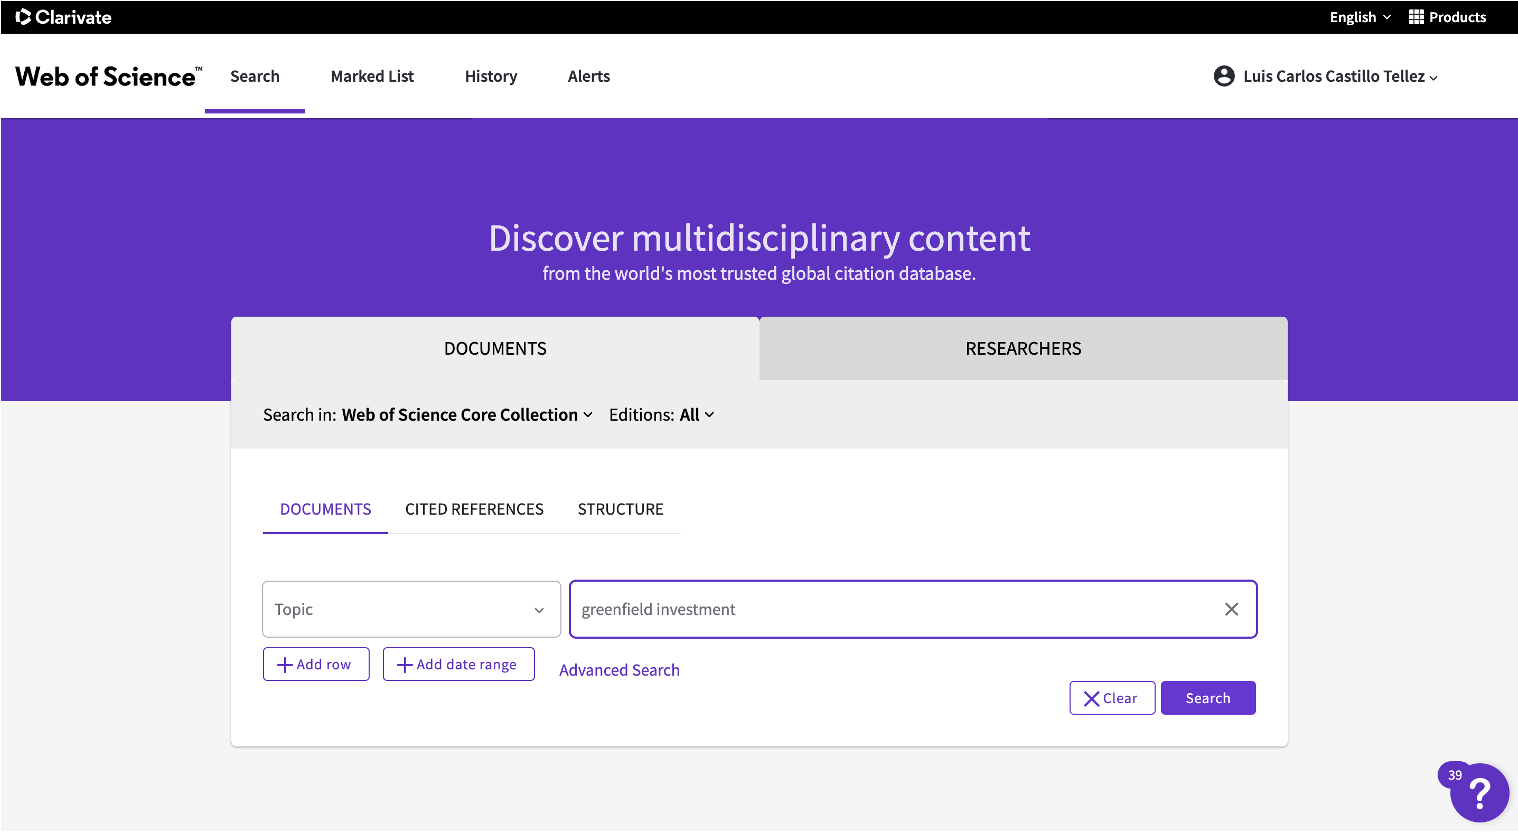
\includegraphics[width=1\linewidth]{C:/Users/eagle/Documents/GitHub/workshop_uniurb/Images/wosplat} \end{center}

\end{document}
